\documentclass[border = 10pt]{standalone}
\usepackage{tikz}
\usepgflibrary{shapes.gates.logic.US} %\usetikzlibrary{arrows, shapes.gates.logic.US, calc}
\usetikzlibrary{circuits.ee.IEC}
\begin{document}


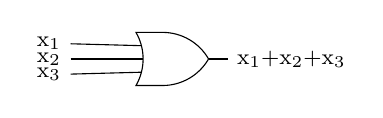
\begin{tikzpicture}
    \node[or gate US, draw, rotate=0, logic gate inputs={normal,normal,normal}] at (1, 0) (trior) {};
    \node (x) at (-0.5,0.2) {\footnotesize \textrm{x}$_1$};
    \node (y) at (-0.5,0) {\footnotesize \textrm{x}$_2$};
    \node (z) at (-0.5,-0.2) {\footnotesize \textrm{x}$_3$};
    \draw (x) -- (trior.input 1);
    \draw (y) -- (trior.input 2);
    \draw (z) -- (trior.input 3);
     \draw (trior.output) --  node[right,fill=white]{\footnotesize x$_1$+x$_2$+x$_3$} ($(trior) + (1, 0)$);

\end{tikzpicture}
\end{document}


